\documentclass{standalone}
\usepackage{graphicx}	
\usepackage{amssymb, amsmath, amsthm}
\usepackage{color}

\usepackage{tikz}
\usetikzlibrary{intersections, backgrounds, fadings}

\definecolor{light}{RGB}{220, 188, 188}
\definecolor{mid}{RGB}{185, 124, 124}
\definecolor{dark}{RGB}{143, 39, 39}
\definecolor{highlight}{RGB}{180, 31, 180}
\definecolor{gray10}{gray}{0.1}
\definecolor{gray20}{gray}{0.2}
\definecolor{gray30}{gray}{0.3}
\definecolor{gray40}{gray}{0.4}
\definecolor{gray60}{gray}{0.6}
\definecolor{gray70}{gray}{0.7}
\definecolor{gray80}{gray}{0.8}
\definecolor{gray90}{gray}{0.9}
\definecolor{gray60}{gray}{0.95}

\begin{document}

\begin{tikzpicture}[scale=0.3]
  \tikzfading[name=fade left, left color=transparent!100, right color=transparent!20]
  \tikzfading[name=fade right, left color=transparent!20, right color=transparent!100]

  \pgfmathsetmacro{\dx}{0}
  
  \draw[white] (-17 + \dx, -12) rectangle (17 + \dx, 12);

  \begin{scope}
    \clip (-13 + \dx, -8) rectangle (13 + \dx, 8);
    \node at (0 + \dx, 0) {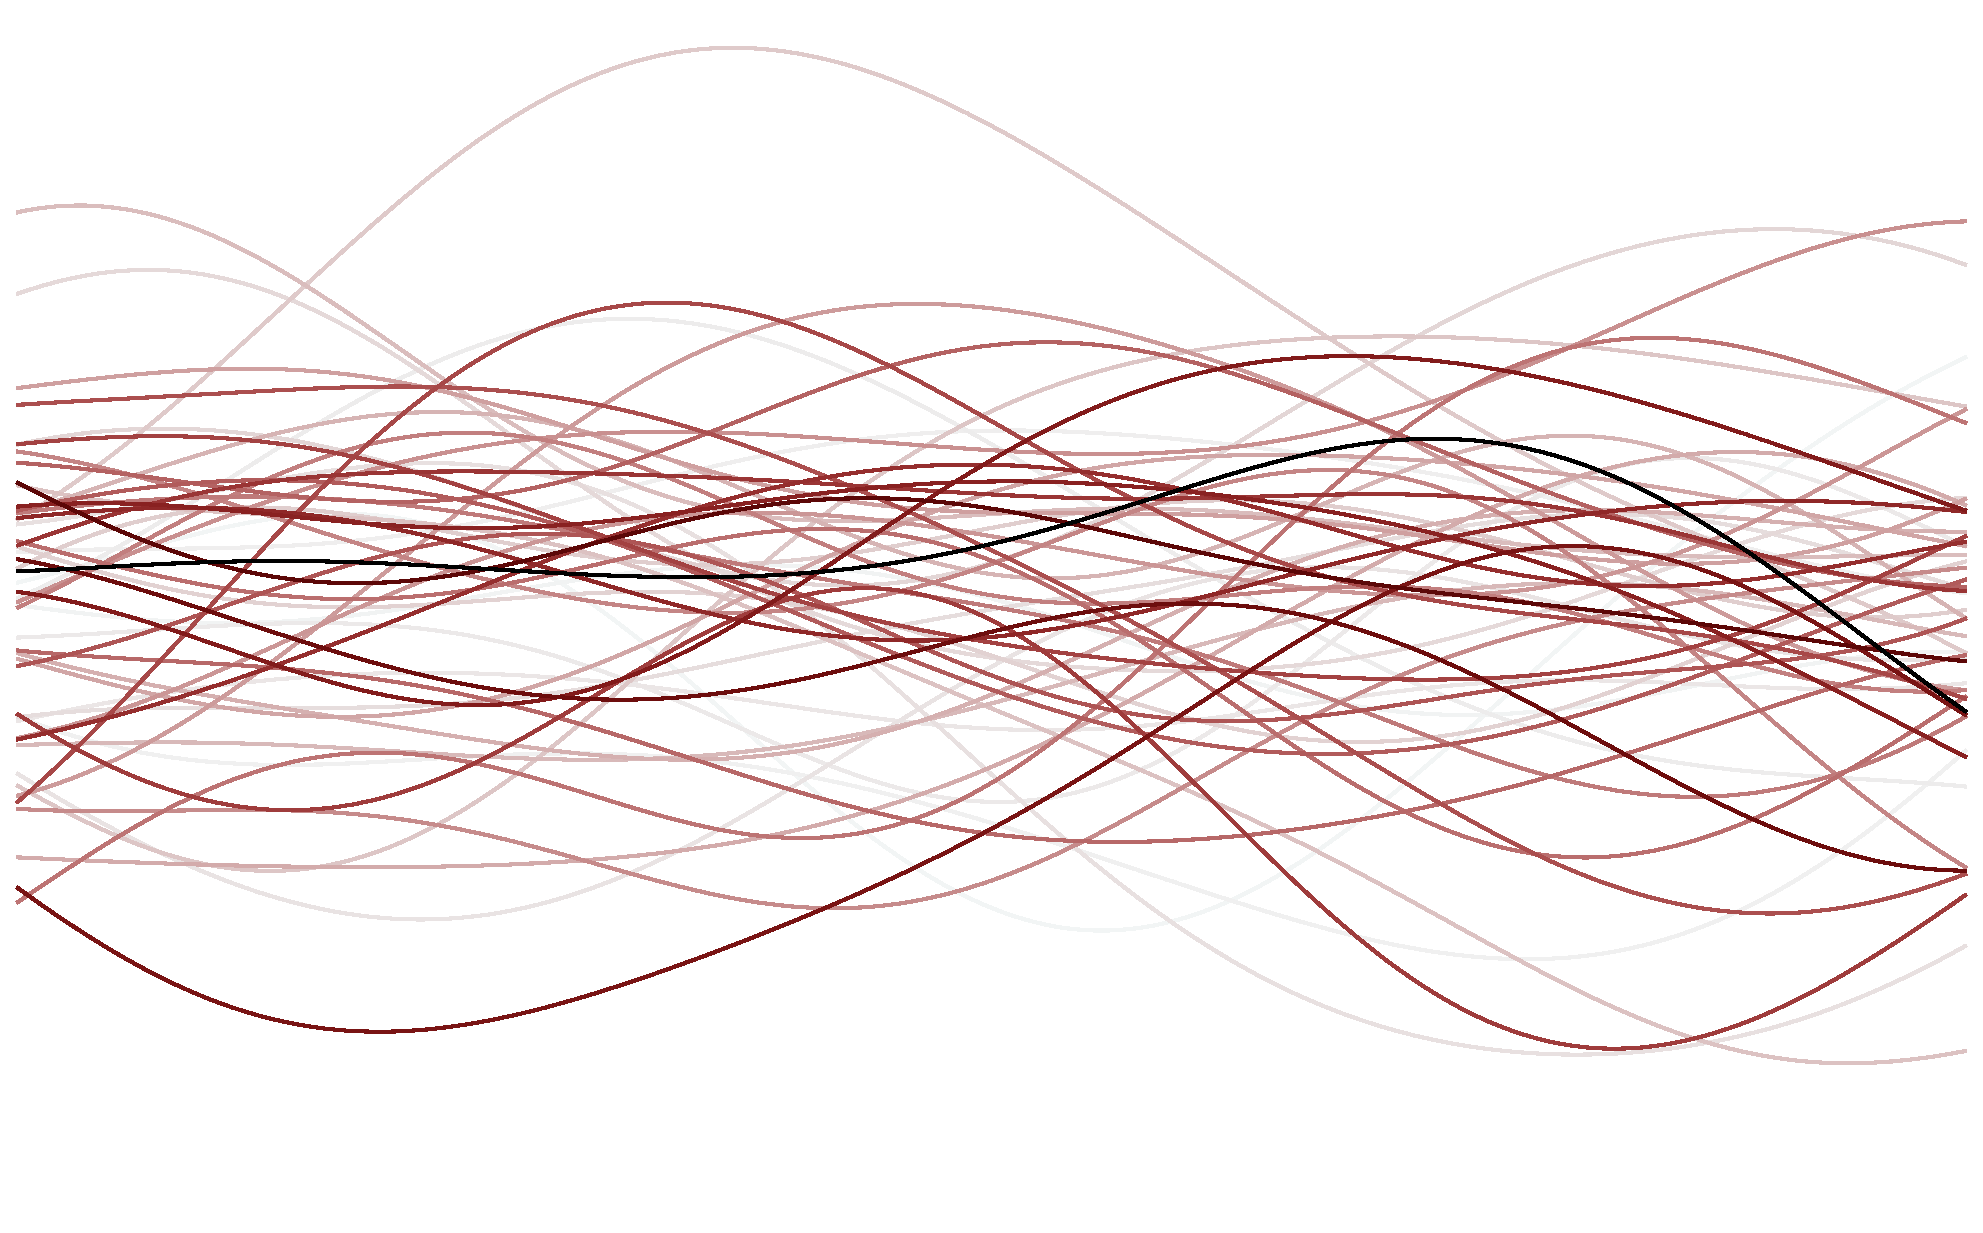
\includegraphics[width=7.8cm]{gp.eps}};
  \end{scope}
  
  \node[] at (0 + \dx, 9.5) { $ \pi(f) = \mathcal{GP}(m, k)$ };
  
  \draw [->, >=stealth, line width=1] (-13 + \dx, -8) -- +(26, 0);
  \draw [->, >=stealth, line width=1] (-13 + \dx, -8.058) -- +(0, 16);
  \node[] at (0 + \dx, -10) { $x$ };
  \node[] at (-15 + \dx, 0) { $f(x)$ };
  
  \pgfmathsetmacro{\dx}{36}
  
  \draw[white] (-17 + \dx, -12) rectangle (17 + \dx, 12);

  \draw[dashed, color=gray70, line width=1] (-8.275 + \dx, -8) -- +(0, 16);
  \node[] at (-8.275 + \dx, -9) { $x_{1}$ };

  \begin{scope}
    \clip (-13 + \dx, -8) rectangle (13 + \dx, 8);
    \node at (0 + \dx, 0) {\includegraphics[width=7.8cm]{gp_uni_proj.eps}};
      
    \pgfmathsetmacro{\x}{-8.275}
    \fill[white, opacity=0.8] (-13 + \dx, -8) rectangle (\x - 0.5 + \dx, 8);      
    \fill[white, path fading=fade right] (\x + \dx, -8) rectangle (\x - 0.5 + \dx, 8);
    \fill[white, path fading=fade left] (\x + \dx, -8) rectangle (\x + 0.5 + \dx, 8);
    \fill[white, opacity=0.8] (\x + 0.5 + \dx, -8) rectangle (13 + \dx, 8);
  \end{scope}
  
  \node[] at (0 + \dx, 9.5) { $ \pi(f(x_{1})) = \text{normal}(m(x_{1}), \sqrt{ k(x_{1}, x_{1}) }) $ };
  
  \draw [->, >=stealth, line width=1] (-13 + \dx, -8) -- +(26, 0);
  \draw [->, >=stealth, line width=1] (-13 + \dx, -8.058) -- +(0, 16);
  \node[] at (0 + \dx, -10) { $x$ };
  \node[] at (-15 + \dx, 0) { $f(x)$ };
 
\end{tikzpicture}

\end{document}  